\documentclass[tikz, margin=3mm]{standalone}
\usepackage{tikz}
\usetikzlibrary{shapes,arrows,calc,positioning}

% From PSLTDSim flow chart - maybe useful (maybe not...)
%\usetikzlibrary{shapes.geometric, arrows, positioning}
%\tikzstyle{arrow} = [thick,->,>=stealth]

\usepackage{amsmath} % for dfrac
\usepackage{comment}
\usepackage{calc}

% Block definition
\tikzset{
    block/.style = {draw, rectangle,
        minimum height=1.2cm,
        minimum width=2cm},
    input/.style = {coordinate,node distance=1cm},
    output/.style = {coordinate,node distance=1cm},
    sum/.style = {draw, circle, node distance=1cm},
}

% Saturation Block
\tikzset{% from https://tex.stackexchange.com/questions/161075/saturation-block
  saturation block/.style={%
    draw, 
    path picture={
      % Get the width and height of the path picture node
      \pgfpointdiff{\pgfpointanchor{path picture bounding box}{north east}}%
        {\pgfpointanchor{path picture bounding box}{south west}}
      \pgfgetlastxy\x\y
      % Scale the x and y vectors so that the range
      % -1 to 1 is slightly shorter than the size of the node
      \tikzset{x=\x*.4, y=\y*.4}
      %
      % Draw annotation
      \draw (-1,0) -- (1,0) (0,-1) -- (0,1); 
      \draw (-1,-.7) -- (-.6,-.7) -- (.6,.7) -- (1,.7);
    }
  }
}

% Deadband block
\tikzset{% from https://tex.stackexchange.com/questions/161075/saturation-block
  deadband block/.style={%
    draw, 
    path picture={
      % Get the width and height of the path picture node
      \pgfpointdiff{\pgfpointanchor{path picture bounding box}{north east}}%
        {\pgfpointanchor{path picture bounding box}{south west}}
      \pgfgetlastxy\x\y
      % Scale the x and y vectors so that the range
      % -1 to 1 is slightly shorter than the size of the node
      \tikzset{x=\x*.4, y=\y*.4}
      %
      % Draw annotation
      \draw (-1,0) -- (1,0) (0,-1) -- (0,1);  % axis
      \draw (-1,1) -- (-.3,.3) -- (-.3,0) -- (.3,0) -- (.3,-.3) -- (1,-1);
	  %\draw (-.3,.3) -- (.3,-.3) ;
    }
  }
}

% Terminal
\tikzstyle{terminal} = [rectangle, rounded corners, minimum width=3cm, minimum height=1cm,text centered, text width=3cm, draw=black]

% Process
\tikzstyle{process} = [rectangle, minimum width=3cm, minimum height=1cm, text centered,text width=4cm, draw=black]

% Decision
\tikzstyle{decision} = [diamond, aspect=1.8, minimum width=2cm, minimum height=1cm, text centered, text width=2cm, draw=black]

% Subprocess
\newcommand\ppbb{path picture bounding box}
\tikzset{
	subprocess/.style = {rectangle, draw=black, 
		minimum width=4.3cm, minimum height=1cm, inner xsep=3mm,
		text width =\pgfkeysvalueof{/pgf/minimum width}-2*\pgfkeysvalueof{/pgf/inner xsep},
		align=flush center,
		path picture={\draw 
			([xshift =2mm] \ppbb.north west) -- ([xshift= 2mm] \ppbb.south west)
			([xshift=-2mm] \ppbb.north east) -- ([xshift=-2mm] \ppbb.south east);
		},% end of path picture
	}
}

% Note
\tikzstyle{note} = [fill, ellipse,fill=gray!20, node distance=4cm, minimum height=1em, text width=3cm, text centered]


\begin{document}
	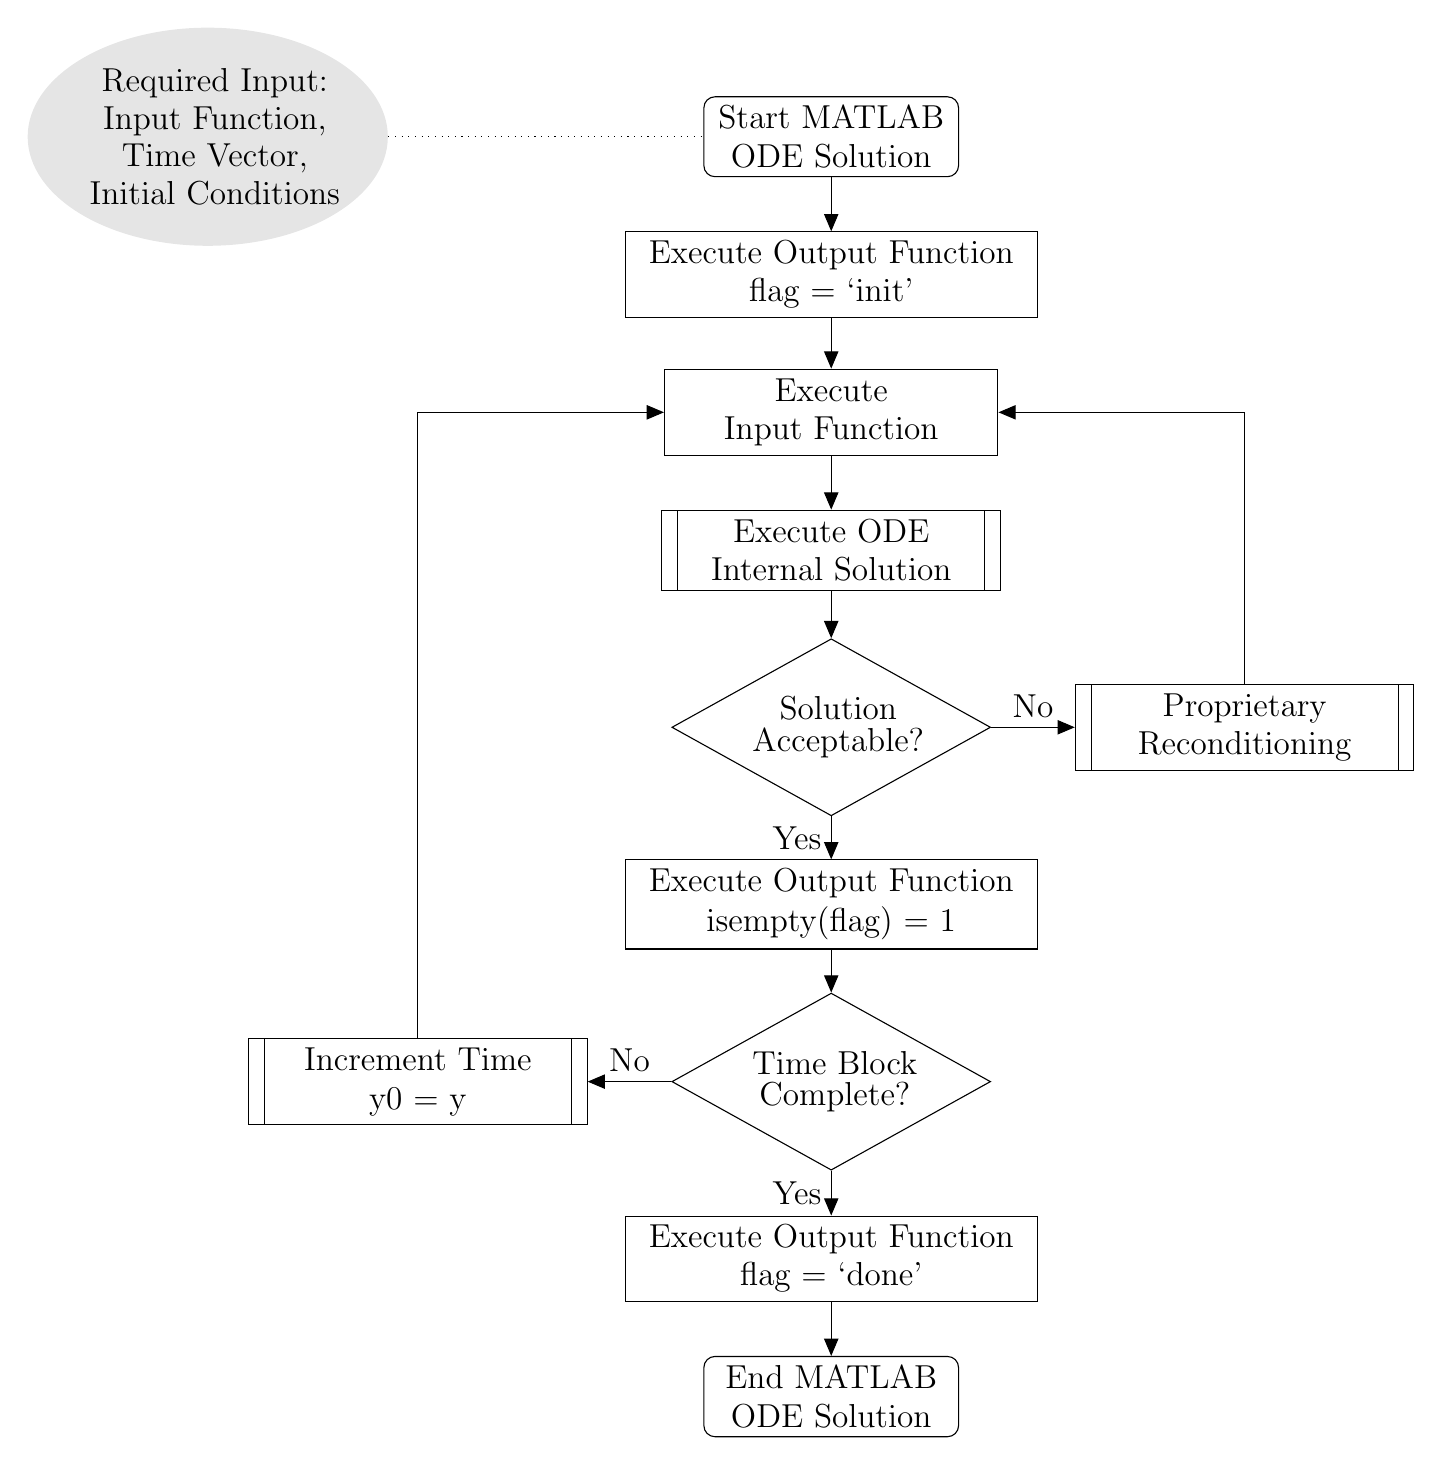
\begin{tikzpicture}[auto, node distance=1.75cm, >=triangle 45, font=\large] % [node distance=1.5cm, font=\large] 
	
	% diagram blocks
	\node (start) [terminal] {Start MATLAB ODE Solution};
	\node (inputNote) [note, left=of start] {\shortstack{Required Input: \\Input Function, \\Time Vector, \\Initial Conditions}};
	\draw [dotted] (inputNote) -> (start);
	
	\node (initFlag) [process, below of=start, text width=5cm] {\shortstack{Execute Output Function\\ flag = `init'}};
	
	\node (inputFcn) [process, below of=initFlag] {Execute \\Input Function}; % returns dx
	%\node (inFcnNote) [note, below right=1cm of inputFcn] {\shortstack{Returned Output: \\Deriviateve Vector}};
	
	\node (odeSln) [subprocess, below of=inputFcn] {Execute ODE Internal Solution}; % black box...
	
	\node (checkSln) [decision, text width=2 cm, yshift=-.5cm, below of=odeSln] {\shortstack{Solution\\Acceptable?}};
	
	\node (recondition) [subprocess, right of=checkSln, xshift=3.5cm] {Proprietary Reconditioning}; % black box...
	
	\node (emptyFlag) [process, below of=checkSln, text width=5cm, yshift=-.5cm] {\shortstack{Execute Output Function\\ isempty(flag) = 1 }};
	
	\node (checkTime) [decision, text width=2 cm, yshift=-.5cm, below of=emptyFlag] {\shortstack{Time Block\\Complete?}};
	
	\node (nextStep) [subprocess, left of=checkTime, xshift=-3.5cm] {Increment Time\\ y0 = y}; 
	
	\node (doneFlag) [process, below of=checkTime, text width=5cm, yshift=-.5cm] {\shortstack{Execute Output Function\\ flag = `done' }};
	
	\node (end) [terminal, below of=doneFlag] {End MATLAB ODE Solution};
	
	%% decision edges
	% Solution Acceptable?
	\draw [->] (checkSln.east) --  node[anchor=south] {No} (recondition);
	\draw [->] (checkSln) --  node[anchor=east] {Yes} (emptyFlag);
	\draw [->] (recondition) |- (inputFcn);
	% Time Over?
	%\draw [-] (checkTime.west) --  node[anchor=south] {No} ($(checkTime.west) + (-2,0)$);
	%\draw [->] ($(checkTime.west) + (-2,0)$) |-  (inputFcn.west);
	\draw [->] (checkTime) -- node[anchor = south] {No} (nextStep);
	\draw [->] (nextStep) |- (inputFcn);
	\draw [->] (checkTime) --  node[anchor=east] {Yes} (doneFlag);
	
	% all other edges
	\draw[->] (start) -- (initFlag);
	\draw[->] (initFlag) -- (inputFcn);
	\draw[->] (inputFcn) -- (odeSln);
	\draw[->] (odeSln) -- (checkSln);
	\draw[->] (emptyFlag) -- (checkTime);
	\draw[->] (doneFlag) -- (end);
	
	\end{tikzpicture} 
\end{document}